\iffalse

INSTRUCTIONS: (if this is not lecture1.tex, use the right file name)

  Clip out the ********* INSERT HERE ********* bits below and insert
appropriate TeX code.  Once you are done with your file, run

  ``latex lecture1.tex''

from a UNIX prompt.  If your LaTeX code is clean, the latex will exit
back to a prompt.  Once this is done, run

  ``dvips lecture1.dvi''

which should print your file to the nearest printer.  There will be
residual files called lecture1.log, lecture1.aux, and lecture1.dvi.
All these can be deleted, but do not delete lecture1.tex.
\fi
%
\documentclass[11pt]{article}
\usepackage{amsfonts}
\usepackage{amsmath}
\usepackage{latexsym}
\usepackage{hyperref}
\usepackage{tikz}

\usepackage{tikz-qtree}
\usetikzlibrary{automata,arrows}

\hypersetup{
    colorlinks=true,
    linkcolor=blue,
    filecolor=magenta,      
    urlcolor=cyan,
}
 
\urlstyle{same}

\setlength{\oddsidemargin}{.25in}
\setlength{\evensidemargin}{.25in}
\setlength{\textwidth}{6in}
\setlength{\topmargin}{-0.4in}
\setlength{\textheight}{8.5in}

\newcommand{\handout}[5]{
   %\renewcommand{\thepage}{#1-\arabic{page}}
   \noindent
   \begin{center}
   \framebox{
      \vbox{
    \hbox to 5.78in { {\bf Data Structures and Algorithms} \hfill #2 }
       \vspace{4mm}
       \hbox to 5.78in { {\Large \hfill #5  \hfill} }
       \vspace{2mm}
       \hbox to 5.78in { {\it #3 \hfill #4} }
      }
   }
   \end{center}
   \vspace*{4mm}
}

\newcommand{\lecture}[3]{\handout{L#1}{#2}{}{}{#1}}

\def\squarebox#1{\hbox to #1{\hfill\vbox to #1{\vfill}}}
\def\qed{\hspace*{\fill}
        \vbox{\hrule\hbox{\vrule\squarebox{.667em}\vrule}\hrule}}
\newenvironment{solution}{\begin{trivlist}\item[]{\bf Solution:}}
                      {\qed \end{trivlist}}
\newenvironment{solsketch}{\begin{trivlist}\item[]{\bf Solution Sketch:}}
                      {\qed \end{trivlist}}
\newenvironment{proof}{\begin{trivlist}\item[]{\bf Proof:}}
                      {\qed \end{trivlist}}

\newtheorem{theorem}{Theorem}
\newtheorem{corollary}[theorem]{Corollary}
\newtheorem{lemma}[theorem]{Lemma}
\newtheorem{observation}[theorem]{Observation}
\newtheorem{remark}[theorem]{Remark}
\newtheorem{proposition}[theorem]{Proposition}
\newtheorem{definition}[theorem]{Definition}
\newtheorem{Assertion}[theorem]{Assertion}
\newtheorem{fact}[theorem]{Fact}
\newtheorem{hypothesis}[theorem]{Hypothesis}
%\newtheorem{observation}[theorem]{Observation}
%\newtheorem{proposition}[theorem]{Proposition}
\newtheorem{claim}[theorem]{Claim}
\newtheorem{assumption}[theorem]{Assumption}

%Put more macros here, as needed.
\newcommand{\al}{\alpha}
\newcommand{\Z}{\mathbb Z}
\newcommand{\jac}[2]{\left(\frac{#1}{#2}\right)}
\newcommand{\set}[1]{\{#1\}}

\def\ppt{{\sf PPT}}
\def\poly{{\sf poly}}
\def\negl{{\sf negl}}
\def\owf{{\sf OWF}}
\def\owp{{\sf OWP}}
\def\tdp{{\sf TDP}}
\def\prg{{\sf PRG}}
\def\prf{{\sf PRF}}

%end of macros
\begin{document}


\fbox{
\vbox{
\begin{flushleft}
Ann,  Bob, Charlie    (\emph{replace with your names})\\  % authors' names
COSC 336  \\  %class
3/19/2020   (\emph{replace with the current date})\\  % date
\end{flushleft}
\center{\Large{\textbf{Assignment 9}}}
%\end{mdframed}
} % end vbox
} % end fbox
\vline

\textbf{Instructions.}
\begin{enumerate}
\item Due  Nov 23.



\item This is a team assignment. Work in teams of 3-4 students.  Submit one assignment per team, with the names of all students making the team.


\item Your programs must be written in Java.

\item Write your programs neatly - imagine yourself grading your program and see if it is easy to read and understand. 
At the very beginning present your algorithm in plain English or in pseudo-code (or both).
Comment your programs reasonably: there is no need to comment lines like "i++" but do include brief comments describing the main purpose of a specific block of lines.

\item  You will submit on Blackboard 3 files. The first file should be a .pdf file  with the short descriptions in English or in pseudocode of the algorithms  for the  programming tasks  you are required to do and the results that you are required to report. Files 2 and 3  will contain the java codes of the program for  task1 and the program for task 2.





%Staple all pages together.  You should have the electronic copy  of your programs with you (for example on a memory stick) because you may be asked to make a demo.

For editing the above document with  Latex, see the template posted on the course website. 
 
           assignment-template.tex	and
           
          assignment-template.pdf


To append in the  latex file  a pdf file, place it  in the same folder and then include them  in the latex file with 
\begin{verbatim}
\includepdf[pages=-,pagecommand={},width=\textwidth]{file.pdf}

\end{verbatim}
To append in the  latex file a .jpg file (for a photo), use 
\begin{verbatim}
\includegraphics[width=\linewidth]{file.jpg}

\end{verbatim}


\end{enumerate}
\newpage





\textbf{Programming Task 1.}
 This is related to Exercise 22.1-5, page 593 in the textbook.   %Note that there are two parts.

Part (a). Write a program  that computes the adjacency list of the directed  graph $G^2$ (defined in the exercise; this is called the square of $G$), given the adjacency list of the directed graph $G$. 
The graph $G^2$ has the same nodes as $G$, and $(u,v)$ is an edge of $G^2$ if and only if there is path of length $1$ or $2$ from $u$ to $v$.

For example if $G$ is the graph on the left, then $G^2$  is the graph on the right.

\begin{tikzpicture}[>=stealth',shorten >=1pt,auto,node distance=2.0cm,scale=0.2][h]
%\begin{tikzpicture}[shorten >=1pt,auto,node distance=2.8cm]][h]
  \node[state] (0) {$0$};
  \node[state] (1) [right of =0] {$1$};
  \node[state] (2) [below of=0] {$2$};
  \

  
  
  \path[->]
    (0) edge  (1)    
    (1) edge  (2) 
  
    ;
   
\end{tikzpicture}
\quad \quad \quad\quad\begin{tikzpicture}[>=stealth',shorten >=1pt,auto,node distance=2.0cm,scale=0.2][h]
%\begin{tikzpicture}[shorten >=1pt,auto,node distance=2.8cm]][h]
  \node[state] (0) {$0$};
  \node[state] (1) [right of =0] {$1$};
  \node[state] (2) [below of=0] {$2$};
  \

  
  
  \path[->]
    (0) edge  (1)    
    (1) edge  (2) 
    (0)   edge (2)
    ;
   
\end{tikzpicture}


For the adjacency list, you \textbf{must} use the Java class \textsf{Adj\_List\_Graph} given in the file \textsf{Adj\_List\_Graph.java} (see \textsf{Test\_Adj.java} for a very simple example of using this class).

You will read the input graph $G$ from a file which contains 2 lines. The first line contains the number $n$ of vertices of the graph. The second line contains a sequence of $n^2$  bits (values $0$ and $1$). The $n$ nodes are labeled $0,1, \ldots, n-1$. If the $i \times n + j$-th  bit in the sequence is $1$, then there is an edge from node $i$ to node $j$, and if the $i \times n + j$-th bit in the sequence is $0$,  then there is no edge from node $i$ to node $j$.

The program has to create the adjacency list of the graph $G^2$ and then use the \textsf{printGraph} function of the class \textsf{Adj\_List\_Graph} to print the edges of $G^2$.

Run your program on two data sets from the files

input-9.1 

input-9.2

Describe briefly your program and report the results in the .pdf file.
\bigskip


\textbf{Programming Task 2.}

Write the program that modifies Breadth First Search  (see for example  the basic version of BFS in Notes 10) in such a way that given an undirected connected graph $G$, and a starting node $s$, it will print for every node $v$ the length of the shortest path from $s$ to $v$ and also the number of shortest paths from $s$ to $v$. Thus, you'll have two arrays $dist$ and $npath$, and for each vertex $v$, at the end of the program, $dist[v]$ will be equal to the length of a shortest path from $s$ to $v$, and $npath[v]$ will be equal to the number of shortest paths from $s$ to $v$.

(For example, if $G_1$ is the first graph below, the length of a shortest path from 1 to 7 is 3, and there are three shortest paths from 1 to 7, namely 

1 - 2 - 5 - 7, 

1 - 3 - 5 - 7 and 

1 - 4 - 6 -7).

So,  $dist[7]=3$, and $npath[7] = 3$.
\medskip


Test your program on the graphs $G_1$ and $G_2$ (see the figures) using $1$ as the starting node and report the results you have obtained for these two graphs. You must use the adjacency list representation of a graph. As in the other programming task, for the adjacency list, you \textbf{must} use the Java class \textsf{Adj\_List\_Graph} given in the file \textsf{Adj\_List\_Graph.java} (see \textsf{Test\_Adj.java} for a very simple example of using this class).



\newpage
 graph $G_1$ 
\medskip



\begin{tikzpicture}[>=stealth',shorten >=1pt,auto,node distance=2.0cm,scale=0.4][h]
%\begin{tikzpicture}[shorten >=1pt,auto,node distance=2.8cm]][h]
  \node[state] (1) {$1$};
  \node[state] (2) [below left of =1] {$2$};
  \node[state] (3) [right of=2] {$3$};
  \node[state] (4) [right of=3] {$4$};
  \node[state] (5) [below of=2] {$5$};
\node[state] (6) [below of=4] {$6$};
\node[state] (7) [below of=5] {$7$};

  
  
  \path[-]
    (1) edge  (2)    
    (1) edge  (3) 
    (1) edge  (4) 
    (2) edge (5)
    (3) edge (5)
    (4) edge (6)
    (5) edge (6)
    (5) edge (7)
    (6) edge (7)
    ;
   
\end{tikzpicture}
\bigskip



graph $G_2$:
\medskip

 \begin{tikzpicture}[>=stealth',shorten >=1pt,auto,node distance=2.0cm,scale=0.4]][h]
%\begin{tikzpicture}[shorten >=1pt,auto,node distance=2.8cm]][h]
  \node[state] (1) {$1$};
  \node[state] (2) [below left of =1] {$2$};
  \node[state] (3) [right of=2] {$3$};
  \node[state] (4) [right of=3] {$4$};
  \node[state] (5) [right of=4] {$5$};
\node[state] (6) [right  of=5] {$6$};
\node[state] (7) [below of=2] {$7$};

  
  
  \path[-]
    (1) edge  (2)    
    (1) edge  (3) 
    (1) edge  (4) 
    (1) edge (5)
    (1) edge (6)
    (7) edge  (2)    
    (7) edge  (3) 
    (7) edge  (4) 
    (7) edge (5)
    (7) edge (6)

    ;
   
\end{tikzpicture}




\end{document}
